This example is presented to introduce \bioptim's ability to provide real-time estimation of biomechanical variables.
The goal was to perform a real-time estimation of dynamically consistent joint kinematics and muscle forces, using a moving horizon estimation (MHE) approach (i.e. an optimization approach that uses a series of measurements observed over time). 
A shoulder elevation motion was performed with a 4-DoFs ($\bf{q}$) arm actuated by 19 Hill-type muscle elements.
The control inputs of the model were the muscle activations ($\bf{a}$).
The MHE implementation consists in splitting the OCP into a succession of smaller one for processing fixed-size subsets of the tracking data moving forward in time. 
Each time one subproblem is solved, a new measurement is added, the oldest one is discarded and a new subproblem is defined. 
Due to their similarities, the solution of the previous OCP is a good initial guess to the new one. 
The dynamical consistency of the final solution is enforced by continuity constraints on the initial state. 
Each objective function (Eq.~\ref{eq:ocp_exMHE}) was written as the sum of three terms: tracking reference joint angles ($\bf{q^*}$), states and muscle activations regularizations (i.e., least-square criteria): 
\begin{figure}[t!]
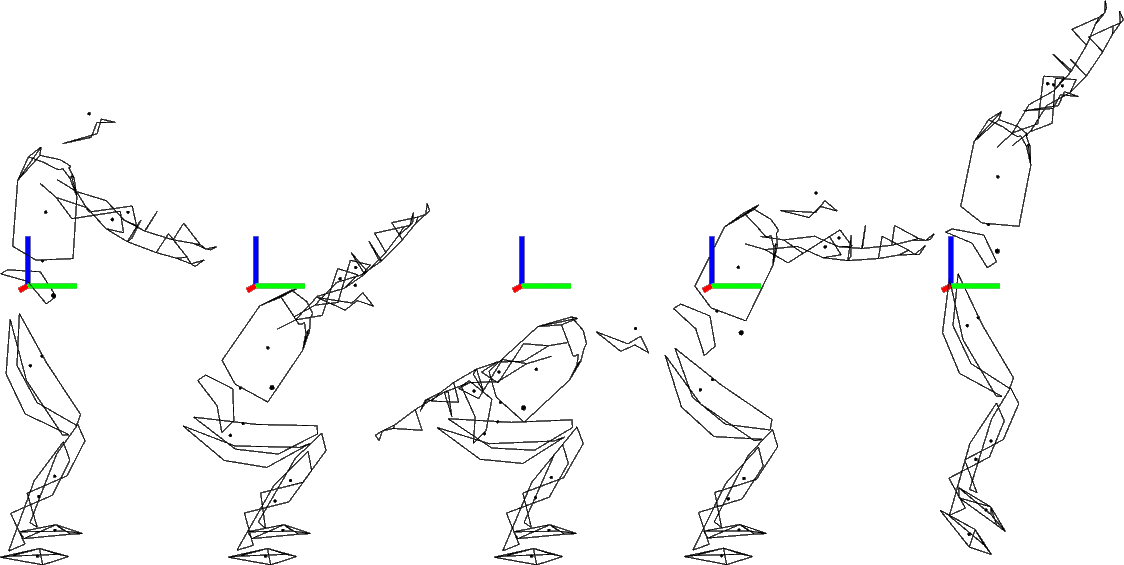
\includegraphics[width=\columnwidth]{figures/kinogramme_jump}
\caption{Snapshots of the push-off phase of a vertical jump (Ex.~\ref{ex:jump}). The avatar reproduces a human-like jump movement. The first four positions represent the first phase of the optimization (i.e., heel and toe in contact with the floor) and the fifth position depicts the end of the second phase (i.e., only the heel in contact with the floor)} 
\label{fig:graph_force_vitesse_longueur}
\end{figure}
\begin{figure*}[t!] 
\centering 
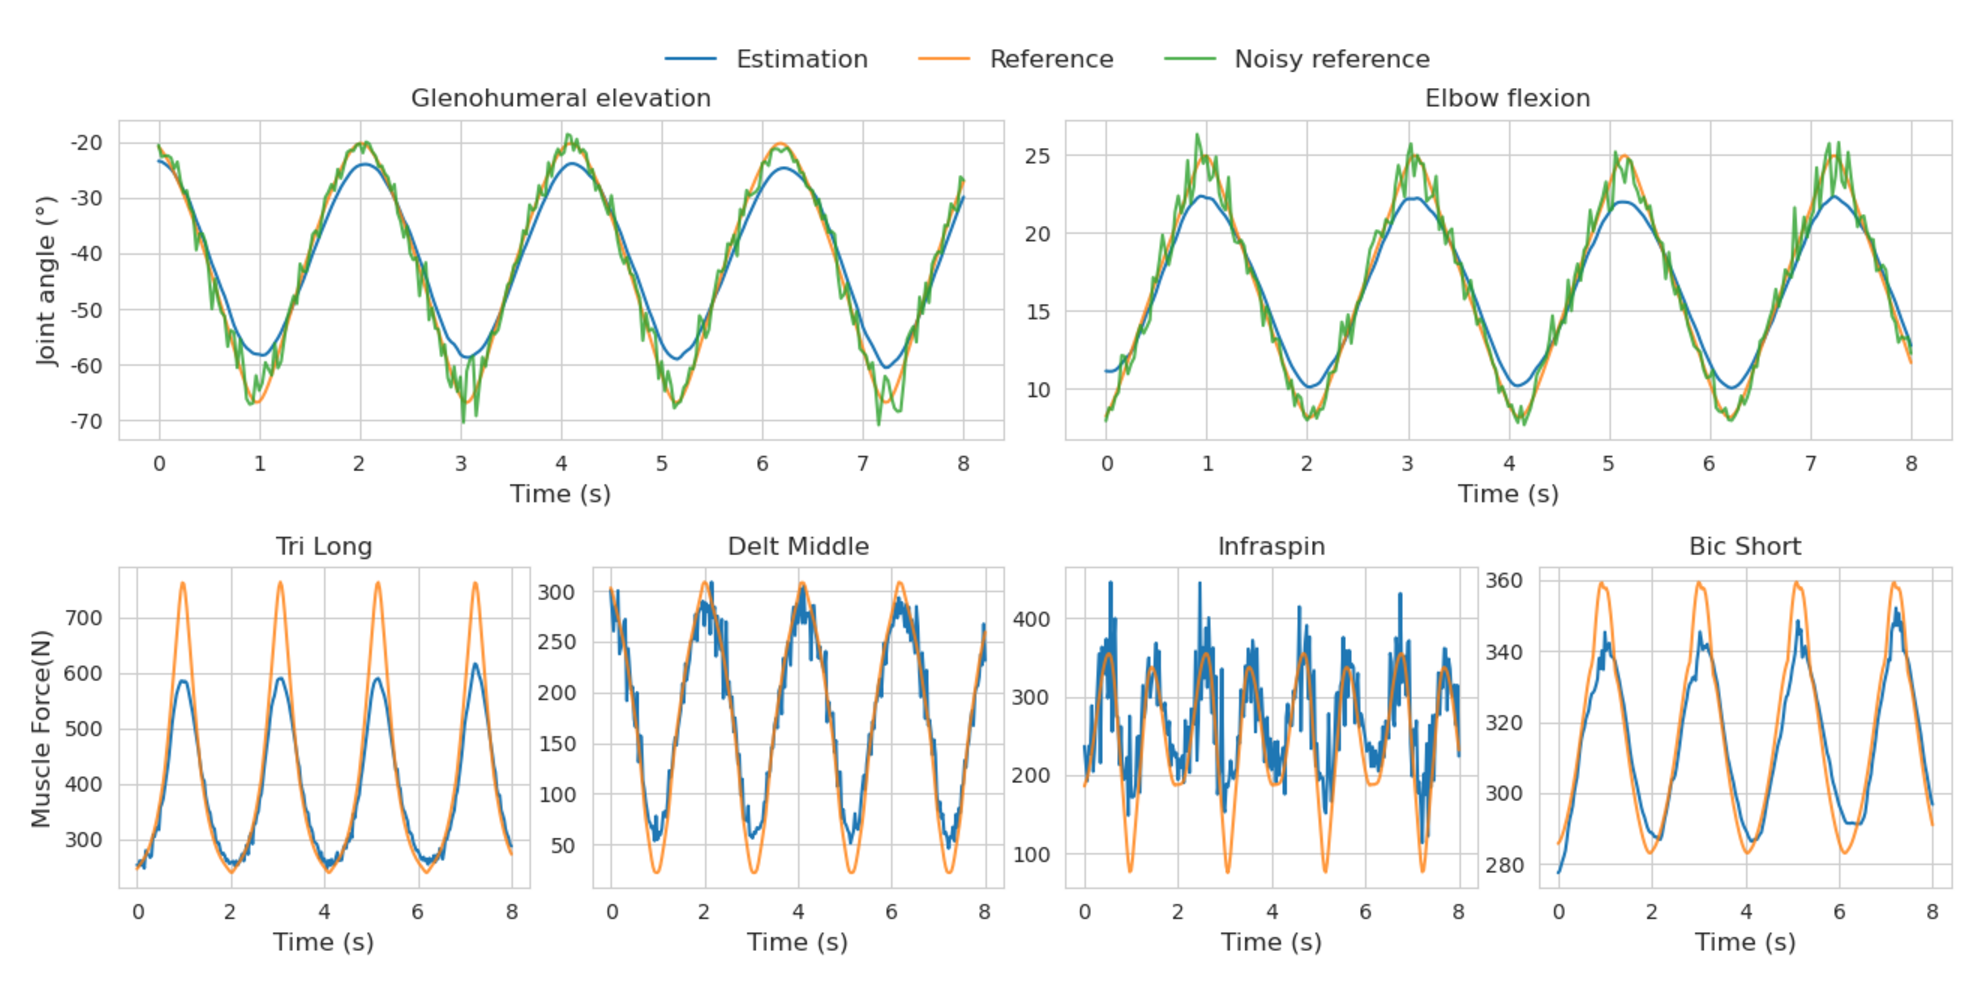
\includegraphics[width=\textwidth]{figures/MHE_results.pdf}\\
\caption{Time series of (1) real-time estimated joint angles (blue), reference joint angle (orange) and noisy reference joint angles (green) of a cyclic motion (up).
(2) Real-time estimated muscle forces (blue) and ground truth muscle forces (orange) of a cyclic motion (bottom) (Ex.~\ref{ex:mhe}).
Only four muscles with significative action (peaks force $>$ 15~N), on the two selected DoFs, are shown.
Muscle abbreviations stand for (from left to right): Triceps Long head, Deltoid Middle, Infraspinatus, Biceps Brachial Short head. (Ex.~\ref{ex:mhe}).} 
\label{fig:MHE_results}
\end{figure*} 
\\ 
\[ 
\resizebox{0.9\columnwidth}{!}{$ 
\begin{aligned}
\mathcal{J} = &\int_t^{t+t_{mhe}}\underbrace{\omega_1´(\|\boldsymbol{q} - \boldsymbol{q^*}\|^{2})}_{\mathtt{TRACK\_STATE}}~ 
+ ~ \underbrace{\omega_2\|\boldsymbol{q\|^2}}_{\mathtt{MIN\_STATE}} 
+ ~ \underbrace{\omega_3\|\boldsymbol{a\|^2}}_{\mathtt{MIN\_ACTIVATION}}~dt, 
\end{aligned}   
$}  
\addtag  
\label{eq:ocp_exMHE}  
\]  

\noindent where $\omega_1 =10^3$, $\omega_2 = 10$, $\omega_3 = 10^2$ and $t_{mhe}$ is duration of each sub-problem. 

In this example, reference data of an $8~s$ series of four arm elevations were generated at 100~Hz, by computer simulation.
A centered Gaussian noise (mean = 0, std = $0.005\:q^*(t)$) was added to $q^*$, to simulate experimental-like joints angle measurements.
Using a windows size of 7 nodes (i.e., 210~ms), the estimator ran at about 33~Hz (one in three reference data frame was sent to the estimator to simulate experimental-like conditions), i.e., two and half times faster than standard biofeedback (13~Hz, \cite{kannape2013self}).
The MHE was able to forecast the movement kinematics with a root mean square error of $1.3\pm0.7^{\circ}$ while providing a realistic estimation of muscle forces close to the ground truth with a root mean square error of $11.1\pm14.9N$ (Fig.~\ref{fig:MHE_results}).

